\section{Trasformata Continua Di Fourier}
    \subsection{Segnali Aperiodici}
        Nel caso di segnali come $x_{(t)}=rect\left(\frac{t}{T}\right)$ non posso usare la $TSF$ posso peró scrivere:
        \[
            x_{(t)} = \lim_{T_0\rightarrow\infty} x_p(t) ,\ x_p(t) = \sum_{n = -\infty}^{\infty} x_{(t-nT_0)} 
        \]
        Passiamo da un analisi a frequenze discrete ad un analisi su tutto lo spettro delle frequenze
        \begin{figure}[H]
            \centering
            \subfloat[Spettro di Ampiezza TSF]{
                    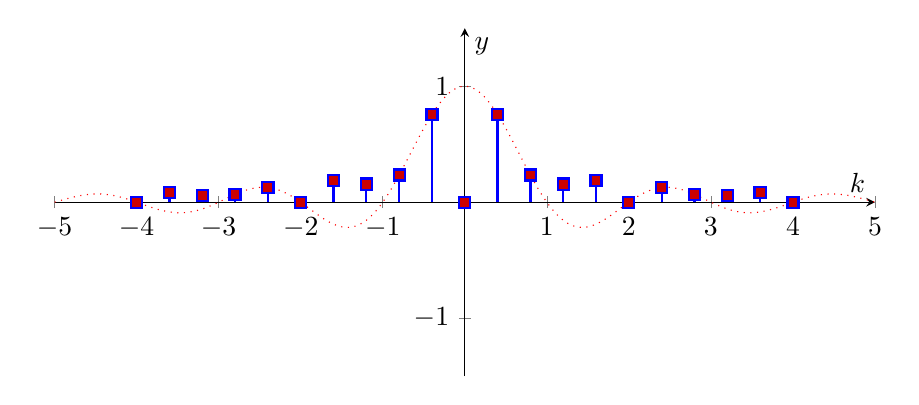
\begin{tikzpicture}
                        \begin{axis}[
                            domain=-5:5,
                            samples=200,
                            axis lines=middle,
                            xlabel=$k$,
                            ylabel=$y$,
                            ymin=-1.5,
                            ymax=1.5,
                            xtick={-5,-4,-3,-2,-1,0,1,2,3,4,5},
                            xticklabels={$-5$,$-4$,$-3$,$-2$,$-1$,$0$,$1$,$2$,$3$,$4$,$5$},
                            ytick={-1, 1},
                            yticklabels={$-1$, $1$},
                            width=12cm,
                            height=6cm
                        ]
                        \addplot [red,dotted, samples = 300] {sin(deg(x*pi))/(x*pi)};
                        \addplot+ [blue, thick, ycomb, samples at={-4,-3.6,-3.2,-2.8,-2.4,-2,-1.6,-1.2,-0.8,-0.4,0,0.4,0.8,1.2,1.6,2,2.4,2.8,3.2,3.6,4}] {abs(sin(deg(x*pi))/(x*pi))};
                        \end{axis}
                    \end{tikzpicture}
                }
                \hfill
                \subfloat[Spettro di Ampiezza TCF]{
                    \begin{tikzpicture}
                        \begin{axis}[
                            domain=-5:5,
                            samples=200,
                            axis lines=middle,
                            xlabel=$f$,
                            ylabel=$y$,
                            ymin=-1.5,
                            ymax=1.5,
                            xtick={-5,-4,-3,-2,-1,0,1,2,3,4,5},
                            xticklabels={$-5$,$-4$,$-3$,$-2$,$-1$,$0$,$1$,$2$,$3$,$4$,$5$},
                            ytick={-1, 1},
                            yticklabels={$-1$, $1$},
                            width=12cm,
                            height=6cm
                        ]
                        \addplot [red,dotted, samples = 300] {sin(deg(x*pi))/(x*pi)};
                        \addplot [blue, thick, samples = 300] {abs(sin(deg(x*pi))/(x*pi))};
                    \end{axis}
                    \end{tikzpicture}
                }
        \end{figure}

    \subsection{Equazioni di Analisi e Sintesi}
        \begin{figure}[H]
            \centering
            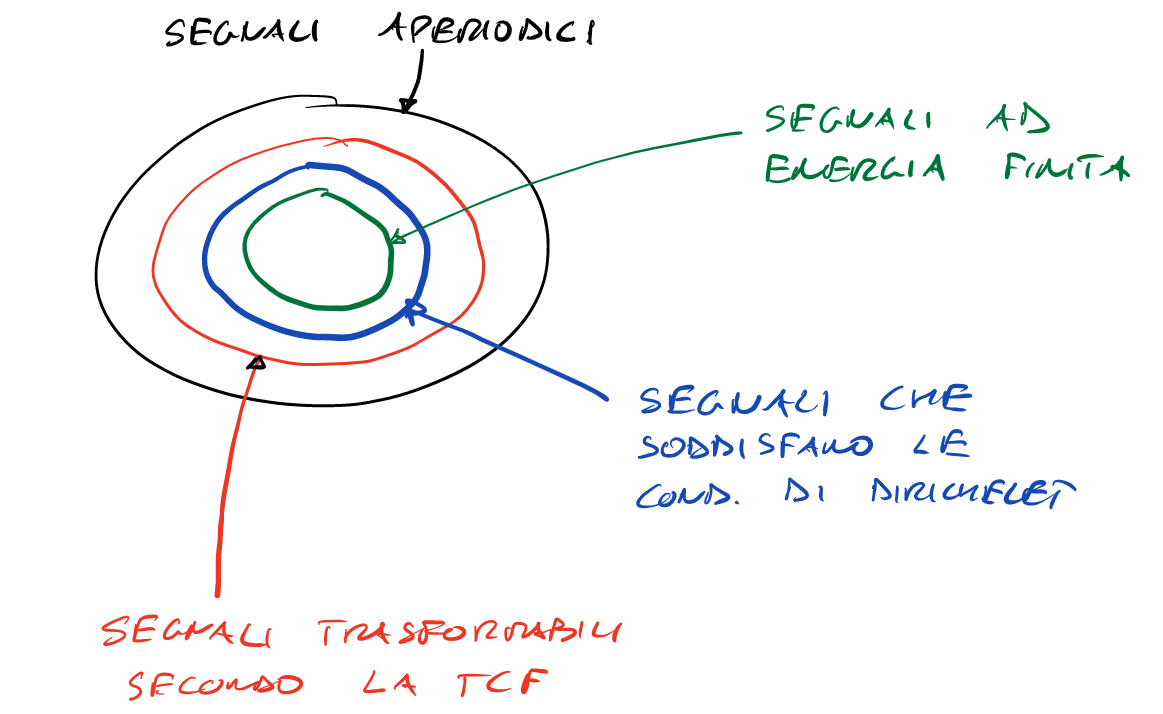
\includegraphics[width=12cm]{media/insiemi_tcf.png}
            \caption{Insiemi dei segnali per tcf}
            \label{fig:segnali aperiodici tcf}
        \end{figure}
        {\subsubsection{Equazione di Analisi}
            \[X_{(f)} = \int_{-\infty}^{\infty} x_{(t)} e^{-j2\pi ft} dt\hspace{0.3cm} Equazione\ di\ analisi \]
            
        \subsubsection{Equazione di Sintesi}
            \[x_{(t)} = \int_{-\infty}^{\infty} X_{(f)} e^{j2\pi ft} df\hspace{0.3cm} Equazione\ di\ sintesi \]
        }
        La $TCF$ gode della biunivocitá
        \begin{align}
            x_{(t)} \rightleftharpoons  X_{(f)}\nonumber \hspace{0.3cm} X_{(f)} \in \mathbb{C}
        \end{align}
        Essendo $X_k$ un numero complesso puó essere rappresentato in forma polare: 
        \[
            X_{(f)} = |X_{(f)}|e^{\angle X_{(f)}}  
        \]
        Si possono rappresentare il modulo (Ampiezza) e la fase tramite grafici che prendono il nome di spettri:
        \begin{figure}[H]
            \centering
            \subfloat[Spettro di Ampiezza]{
                    \begin{tikzpicture}
                        \begin{axis}[
                            domain=-5:5,
                            samples=200,
                            axis lines=middle,
                            xlabel=$f$,
                            ylabel=$y$,
                            ymin=-1.5,
                            ymax=1.5,
                            xtick={-5,-4,-3,-2,-1,0,1,2,3,4,5},
                            xticklabels={$-5$,$-4$,$-3$,$-2$,$-1$,$0$,$1$,$2$,$3$,$4$,$5$},
                            ytick={-1, 1},
                            yticklabels={$-1$, $1$},
                            width=12cm,
                            height=6cm
                        ]
                        \addplot [red,dotted, samples = 300] {sin(deg(x*pi))/(x*pi)};
                        \addplot [blue, thick, samples = 300] {abs(sin(deg(x*pi))/(x*pi))};
                    \end{axis}
                    \end{tikzpicture}
                }
            \hfill
            \subfloat[Spettro di Fase]{
                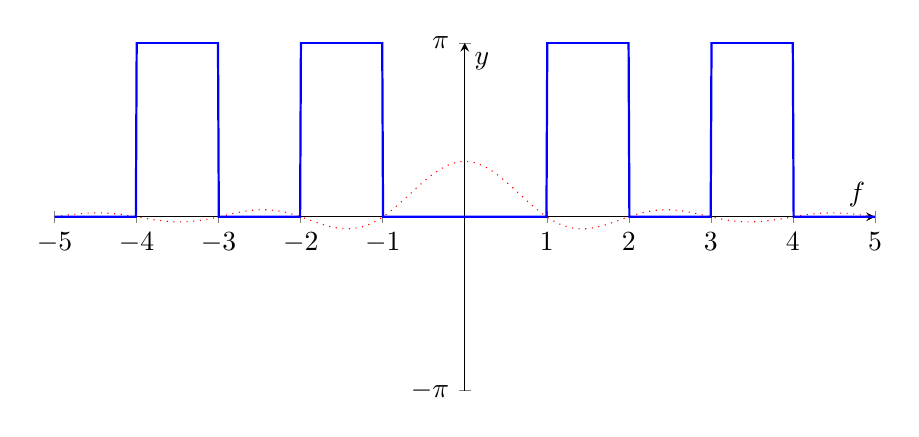
\begin{tikzpicture}
                    \begin{axis}[
                        domain=-5:5,
                        samples=200,
                        axis lines=middle,
                        xlabel=$f$,
                        ylabel=$y$,
                        ymin=-pi,
                        ymax=pi,
                        xtick={-5,-4,-3,-2,-1,0,1,2,3,4,5},
                        xticklabels={$-5$,$-4$,$-3$,$-2$,$-1$,$0$,$1$,$2$,$3$,$4$,$5$},
                        ytick={-pi, pi},
                        yticklabels={$-\pi$, $\pi$},
                        width=12cm,
                        height=6cm
                    ]
                    \addplot [red,dotted, samples = 300] {sin(deg(x*pi))/(x*pi)};
                    \addplot [blue, thick, samples = 1000] {rad(atan2(0,sin(deg(x*pi))/(x*pi)))};
                    \end{axis}
                \end{tikzpicture}
            }
            \caption{Spettro del segnale TCF}
        \end{figure}
        lo spettro di Ampiezza gode della \textbf{simmetria pari} rispetto alle ascisse quindi é \textbf{sempre positivo e continuo}, mentre lo spettro di fase della \textbf{simmetria dispari}, 
        questa propietá é chiamata \textbf{Simmetria Hermitiana}

        \subsubsection{TCF di una $Arect\left(\frac{t}{T}\right)$}
            $x_{(t)} = A\hspace{0.1cm}rect\left(\frac{t}{T}\right)$
            \begin{figure}[H]
                \centering
                \begin{tikzpicture}
                    \begin{axis}[
                        xlabel=$x$,
                        ylabel=$y$,
                        xmin=-5,
                        xmax=5,
                        ymin=-0.5,
                        ymax=4,
                        ytick = {1.5},
                        xtick={-1.5, 0, 1.5},
                        xticklabels={$-\frac{T}{2}$, $0$, $\frac{T}{2}$},
                        yticklabels = {$A$},
                        yticklabel style = {yshift=5pt,xshift=4pt}, 
                        axis lines=middle,
                        thick,
                        domain=-5:5,
                        samples=100,
                        width=8cm,
                        height=4cm
                    ]
                    \addplot [const plot,red, thick] coordinates{(-1.5,1.5)(1.5,1.5)};
                    \addplot [const plot,red, thick] coordinates{(-1.5,0)(-1.5,1.5)};
                    \addplot [const plot,red, thick] coordinates{(1.5,0)(1.5,1.5)};
                    \addplot [const plot,red, thick] coordinates{(5,0)(1.5,0)};
                    \addplot [const plot,red, thick] coordinates{(-5,0)(-1.5,0)};
                    \end{axis}
                  \end{tikzpicture}
                \caption{$A\hspace{0.1cm}rect\left(\frac{t}{T}\right)$}
                \label{fig:grafo rect nella tcf}
            \end{figure}
            $X_{(f)} = ? :$
            \begin{align}
                X_{(f)} & = \int_{-\infty}^{\infty} x_{(t)} e^{-j2\pi ft} dt \nonumber = \int_{-\frac{T}{2}}^{\frac{T}{2}} A\hspace{0.1cm}rect\left(\frac{t}{T}\right) e^{-j2\pi ft} dt \nonumber\\ 
                        & = A \int_{-\frac{T}{2}}^{\frac{T}{2}} e^{-j2\pi ft} dt = -\frac{A}{j2\pi f} \eval{e^{-j2\pi ft}}_{-\frac{T}{2}}^{\frac{T}{2}} =-\frac{A}{j2\pi f} \left(e^{-j\pi fT} - e^{j\pi fT}\right) \nonumber\\
                        & = \frac{A\color{purple}{T}}{\pi f} \left(\frac{e^{j\pi fT} - e^{-j\pi fT}}{2j}\right) = \frac{A{\color{purple}T}\sin(\pi fT)}{\pi f\color{purple}{T}} = AT sinc(fT) =  X_{(f)} \nonumber 
            \end{align}
            \[
                A\hspace{0.1cm}rect\left(\frac{t}{T}\right) \rightleftharpoons AT sinc(fT)
            \]
            La sinc si annulla in $\frac{k}{T},\ k\in \mathbb{Z}$. Notiamo anche come la funzione di partenza sia reale e pari la TCF rispetti \ref{Parita}(si?):
            \begin{figure}[H]
                \centering

            \subfloat[Spettro di Ampiezza]{
                \begin{tikzpicture}
                    \begin{axis}[
                        domain=-5:5,
                        samples=200,
                        axis lines=middle,
                        xlabel=$f$,
                        ylabel=$y$,
                        ymin=-1.5,
                        ymax=1.5,
                        xtick={-5,-4,-3,-2,-1,0,1,2,3,4,5},
                        xticklabels={$-\frac{5}{T}$,$-\frac{4}{T}$,$-\frac{3}{T}$,$-\frac{2}{T}$,$-\frac{1}{T}$,$0$,$\frac{1}{T}$,$\frac{2}{T}$,$\frac{3}{T}$,$\frac{4}{T}$,$\frac{5}{T}$},
                        ytick={-1, 1},
                        yticklabels={$-1$, $1$},
                        width=12cm,
                        height=6cm
                    ]
                    \addplot [red,dotted, samples = 300] {sin(deg(x*pi))/(x*pi)};
                    \addplot [blue, thick, samples = 300] {abs(sin(deg(x*pi))/(x*pi))};
                \end{axis}
                \end{tikzpicture}
                }
            \hfill
            \subfloat[Spettro di Fase]{
                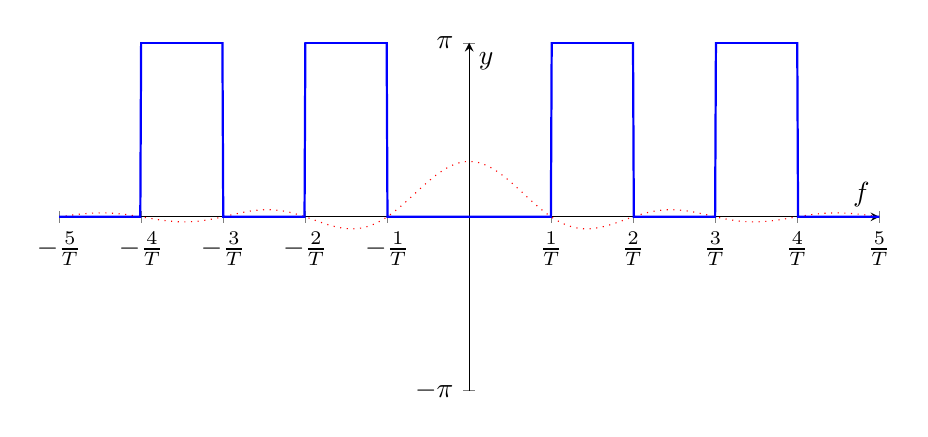
\begin{tikzpicture}
                    \begin{axis}[
                        domain=-5:5,
                        samples=200,
                        axis lines=middle,
                        xlabel=$f$,
                        ylabel=$y$,
                        ymin=-pi,
                        ymax=pi,
                        xtick={-5,-4,-3,-2,-1,0,1,2,3,4,5},
                        xticklabels={$-\frac{5}{T}$,$-\frac{4}{T}$,$-\frac{3}{T}$,$-\frac{2}{T}$,$-\frac{1}{T}$,$0$,$\frac{1}{T}$,$\frac{2}{T}$,$\frac{3}{T}$,$\frac{4}{T}$,$\frac{5}{T}$},
                        ytick={-pi, pi},
                        yticklabels={$-\pi$, $\pi$},
                        width=12cm,
                        height=6cm
                    ]
                    \addplot [red,dotted, samples = 300] {sin(deg(x*pi))/(x*pi)};
                    \addplot [blue, thick, samples = 1000] {rad(atan2(0,sin(deg(x*pi))/(x*pi)))};
                    \end{axis}
                \end{tikzpicture}
            }
            \end{figure}

    \subsection{Propietá}
        Come per la TSF vale che al variare del periodo della funzione $T$:
            \begin{itemize}
                \item Se $T\uparrow$ aumenta $ \rightarrow f\downarrow$ diminuisce e si stringe lo spettro  
                \item Se $T\downarrow$ diminuisce $ \rightarrow f\uparrow$ aumenta e si allarga lo spettro  
            \end{itemize}
        Inoltre come si puó evincere dal successivo Teorema della Dualitá \ref{Dualita}:
            \begin{itemize}
                \item Una funzione limitata (finita) nel tempo ha uno spettro nella frequenza illimitato $\rightarrow$ sono i segnali fisici   
                \item Una funzione illimitata nel tempo ha uno spettro nella frequenza limitato (finito)
            \end{itemize}

        \subsubsection{Simmetria hermitiana}\label{Simmetria Hermitiana}
            \begin{align}
                Ip&: x_{(t)}\ reale \nonumber \\
                Th&: X_{(f)}\ hermitiana \nonumber \\ 
                X_{(-f)} &= X_{(f)}^{*} \rightarrow
                    \begin{cases}
                        |X_{(f)}| = |X_{(-f)}| \hspace{0.3cm} & Simmetria\ Pari \\
                        \angle X_{(-f)} = -\angle X_{(f)}\hspace{0.3cm} & Simmetria\ Dispari
                    \end{cases} \nonumber
            \end{align}

        \subsubsection{Paritá}\label{Parita}
            \begin{align}
                Ip&: x_{(t)}\ reale\ e\ pari  \nonumber \\
                Th&: X_{(f)}\ reale\ e\ pari \nonumber  
            \end{align}

        \subsubsection{Disparitá}\label{Disparita}
            \begin{align}
                Ip&: x_{(t)}\ reale\ e\ dispari  \nonumber \\
                Th&: X_{(f)}\ immaginaria\ e\ dispari \nonumber 
            \end{align}

    \subsection{Teoremi relativi alla TCF}
        \subsubsection{Linearitá}\label{Linearita}
            $Ip: x_{(t)} = \alpha x_{1(t)} + \beta x_{2(t)}$\\        
            $Th: X_{(f)} = \alpha X_{1(f)} + \beta X_{2(f)}$\\ 
            Dimostrazione:
            \begin{align}
                X_{(f)} & = \int_{-\infty}^{\infty} (\alpha x_{1(t)} + \beta x_{2(t)}) e^{-j2\pi ft} dt \nonumber \\
                        & = \alpha \int_{-\infty}^{\infty} x_{1(t)} e^{-j2\pi ft} dt + \beta \int_{-\infty}^{\infty}  x_{2(t)} e^{-j2\pi ft} dt  \nonumber \\
                        & = \alpha X_{1(f)} + \beta X_{2(f)} \nonumber
            \end{align}

            Esempio:
                {   
                    \begin{align}
                        x_{(t)} &= A rect\left(\frac{t}{2T}\right) + Brect\left(\frac{t}{T}\right)\nonumber \\   
                        X_{(f)} &= A X_{1(f)} + B X_{2(f)} = 2AT sinc(2Tf) + BT sinc(Tf) \nonumber \\
                        X_{1(f)} &= 
                        \begin{cases}
                            X_{1(f)} = A rect\left(\frac{t}{T^\prime}\right) \rightleftharpoons^{TCF} T^\prime sinc(T^\prime f) \Rightarrow X_{1(f)} =2Tsinc(2Tf) \\
                            T^\prime = 2T
                        \end{cases} \nonumber
                    \end{align}
                    \begin{figure}[H]
                        \centering
                        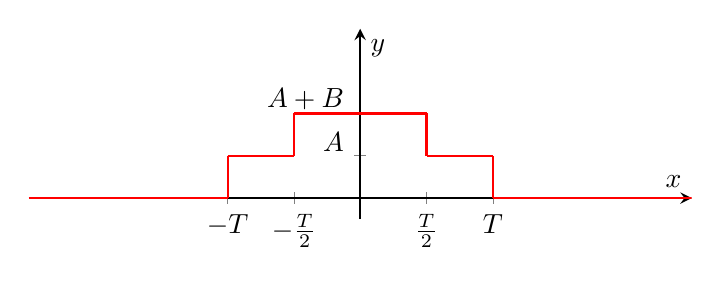
\begin{tikzpicture}
                            \begin{axis}[
                                xlabel=$x$,
                                ylabel=$y$,
                                xmin=-5,
                                xmax=5,
                                ymin=-0.5,
                                ymax=4,
                                ytick = {1,2},
                                yticklabels = {$A$,$A+B$},
                                xtick={-2,-1, 0, 1,2},
                                xticklabels={$-T$,$-\frac{T}{2}$, $0$, $\frac{T}{2}$,$T$},
                                yticklabel style = {yshift=5pt}, 
                                axis lines=middle,
                                thick,
                                domain=-5:5,
                                samples=100,
                                width=10cm,
                                height=4cm
                            ]
                            
                            \addplot [const plot,red, thick] coordinates{(-2,1)(-1,1)};
                            \addplot [const plot,red, thick] coordinates{(2,1)(1,1)};

                            \addplot [const plot,red, thick] coordinates{(1,1)(1,2)};
                            \addplot [const plot,red, thick] coordinates{(-1,1)(-1,2)};
                            \addplot [const plot,red, thick] coordinates{(-1,2)(1,2)};
                            
                            \addplot [const plot,red, thick] coordinates{(-2,0)(-2,1)};
                            \addplot [const plot,red, thick] coordinates{(2,0)(2,1)};


                            \addplot [const plot,red, thick] coordinates{(5,0)(2,0)};
                            \addplot [const plot,red, thick] coordinates{(-5,0)(-2,0)};
                            \end{axis}
                          \end{tikzpicture}
                        \caption{Segnale rettangolo}
                        \label{fig:es linearita}
                    \end{figure}                    
                }
                

        \subsubsection{Dualitá}\label{Dualita}
            $Ip: x_{(t)} \rightleftharpoons^{TCF} X_{(f)}$\\        
            $Th: X_{(t)} \rightleftharpoons^{TCF} x_{(-f)}$ 
            Dimostrazione:
            \begin{align}
                X_{(f)} & = \int_{-\infty}^{\infty} x_{(t)} e^{-j2\pi ft} dt = Sost. \begin{cases}
                    t \rightarrow f\\
                    f \rightarrow t
                \end{cases} \Rightarrow  X_{(t)} = \int_{-\infty}^{\infty} x_{(f)} e^{-j2\pi tf} df \nonumber \\
                        & =Sost.\ (f^\prime = -f) \Rightarrow  X_{(t)} = \int_{-\infty}^{\infty} x_{(-f^\prime)} e^{-j2\pi t(-f^\prime)} df^\prime\nonumber \\
                        & =\int_{-\infty}^{\infty} x_{(-f^\prime)} e^{j2\pi tf^\prime} df^\prime= ACTF[x_{(-f)}] = c.v.d.  \nonumber
            \end{align}
            Esempio:\\
                {
                    $x_{(t)}=Asinc(Bt) \Rightarrow X_{(f)} = \int_{-\infty}^{\infty}A sinc(Bt)e^{-j2\pi ft}dt$ \\
                    Applico la dualitá:
                    \begin{align}
                        A rect\left(\frac{t}{T}\right) &\rightleftarrows ATsinc(Tf) \nonumber \\
                        ATsinc(Tt) &\rightleftarrows A rect\left(\frac{-f}{T}\right) \nonumber
                    \end{align}
                    Se voglio una durata generica(rivedere):
                    \begin{align}
                        Sostituisco\ &B=T \nonumber \\
                        ABsinc(Bt) &\rightleftarrows A rect\left(\frac{f}{B}\right) \nonumber \\
                        &\Downarrow \nonumber \\
                        Asinc(Bt) &\rightleftarrows \frac{A}{B}rect\left(\frac{f}{B}\right) \nonumber 
                    \end{align}
                }

        \subsubsection{Ritardo}\label{Ritardo}
            $Ip: x_{(t)} \rightleftharpoons^{TCF} X_{(f)},\ y_{(t)} = x_{(t-to)}$\\        
            $Th: Y_{(f)} \rightleftharpoons^{TCF} y_{(t)} = X_{(f)}e^{-j2\pi ft_0}$\\ 
            Dimostrazione:
            \begin{align}
                Y_{(f)} & = \int_{-\infty}^{\infty} y_{(t)} e^{-j2\pi ft} dt = \int_{-\infty}^{\infty} x_{(t-t_0)} e^{-j2\pi tf} dt \nonumber \\
                        & =Sost.\ (t^\prime = t-t_0) \Rightarrow  Y_{(f)} = \int_{-\infty}^{\infty} x_{(t^\prime)} e^{-j2\pi f(t^\prime+t_0)} dt^\prime \nonumber \\
                        & =\int_{-\infty}^{\infty} x_{(t^\prime)} e^{-j2\pi ft^\prime}e^{-j2\pi ft_0} dt^\prime= X_{(f)}e^{-j2\pi ft_0}\ c.v.d.  \nonumber
            \end{align}
            {\em Osservazione:}
                \begin{itemize}
                    \item Un ritardo nel tempo introduce una componente solo di fase che cresce lienarmente con la frequenza
                    \item Un esponenziale nel tempo introduce un ritardo nel dominio della frequenza $x_{(t)}e^{-j2\pi f_0t} \rightarrowtail X_{(f-f_0)}$, vedi \ref{Modulazione con Esponenziale Complesso}
                \end{itemize}
            Esempio:\\
                {
                    $x_{0(t)} = A rect\left(\frac{t}{T}\right) \rightarrow x_{(t)}=x_{0(t-t_0)}\hspace{0.3cm} t_0 = \frac{T}{2}$
                    \begin{figure}[H]
                        \centering
                        \begin{tikzpicture}
                            \begin{axis}[
                                xlabel=$t$,
                                ylabel=$y$,
                                xmin=-5,
                                xmax=5,
                                ymin=-0.5,
                                ymax=4,
                                ytick = {1.5},
                                yticklabels = {$A$},
                                yticklabel style = {yshift=8pt,xshift=4pt}, 
                                xtick={-1,0,1,2},
                                xticklabels={$-\frac{T}{2}$,$0$,$\frac{T}{2}$,$T$},
                                axis lines=middle,
                                thick,
                                domain=-5:5,
                                samples=100,
                                width=10cm,
                                height=5cm
                            ]
                            
                            \addplot [const plot, blue] coordinates{(-1,1.5)(1,1.5)};
                            \addplot [const plot, blue] coordinates{(-1,0)(-1,1.5)};
                            \addplot [const plot, blue] coordinates{(1,0)(1,1.5)};
                            
                            \addplot [const plot, purple] coordinates{(0,1.5)(2,1.5)};
                            \addplot [const plot, purple] coordinates{(0,0)(0,1.5)};
                            \addplot [const plot, purple] coordinates{(2,0)(2,1.5)};
                            
                            \end{axis}
                        \end{tikzpicture}
                        \caption{{\color{blue}$x_{0(t)}$}, {\color{purple}$x_{(t)}$}}
                        \label{fig:ritardo rect}
                    \end{figure}
                    \[
                        X_{(f)} = X_{0(f)}e^{-j2\pi f\frac{T}{2}} = AT sinc(Tf) e^{-j\pi fT}    
                    \]

                    \begin{figure}[H]
                        \centering
                        \subfloat[Ampiezza con ritardo]{
                            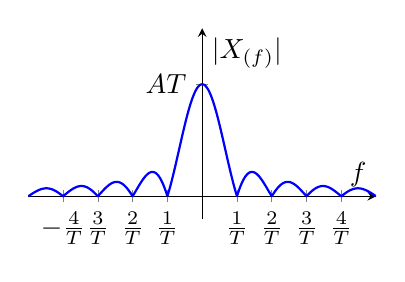
\begin{tikzpicture}
                                \begin{axis}[
                                    domain=-5:5,
                                    samples=200,
                                    axis lines=middle,
                                    xlabel=$f$,
                                    ylabel=$|X_{(f)}|$,
                                    ytick = {1},
                                    yticklabels = {$AT$},
                                    xtick = {-4,-3,-2,-1,0,1,2,3,4},
                                    xticklabels = {$-\frac{4}{T}$,$\frac{3}{T}$,$\frac{2}{T}$,$\frac{1}{T}$,$0$,$\frac{1}{T}$,$\frac{2}{T}$,$\frac{3}{T}$,$\frac{4}{T}$},
                                    ymin=-0.2,
                                    ymax=1.5,
                                    width=6cm,
                                    height=4cm
                                ]
                                \addplot [blue, thick, samples = 500] {abs(sin(deg(x*pi))/(x*pi))};
                                \end{axis}
                            \end{tikzpicture}
                            \label{fig:Ampiezza}
                        }
                        \hfill
                        \subfloat[Fase con ritardo]{
                                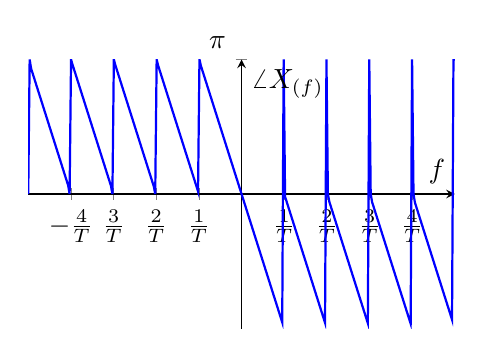
\begin{tikzpicture}
                                    \begin{axis}[
                                        domain=-5:5,
                                        samples=200,
                                        axis lines=middle,
                                        xlabel=$f$,
                                        ylabel=$\angle X_{(f)}$,
                                        ymin=-pi,
                                        ymax=pi,
                                        xtick = {-4,-3,-2,-1,0,1,2,3,4},
                                        xticklabels = {$-\frac{4}{T}$,$\frac{3}{T}$,$\frac{2}{T}$,$\frac{1}{T}$,$0$,$\frac{1}{T}$,$\frac{2}{T}$,$\frac{3}{T}$,$\frac{4}{T}$},
                                        ytick={pi},
                                        yticklabel style = {yshift=6pt}, 
                                        yticklabels={$\pi$},
                                        width=7cm,
                                        height=5cm
                                    ]
                                    \addplot [blue, thick, samples = 300] {rad(atan2((-((sin(deg(pi*x)))^2)/(pi*x)),((cos(deg(pi*x))*sin(deg(pi*x)))/(pi*x))))};
                                    \end{axis}
                                \end{tikzpicture}
                            \label{fig:fase}
                        }
                        \caption{Spettro della $rect$ con ritardo}
                    \end{figure}
                    Il \LaTeX{} sbaglia e aggiunge le spike nelle $f$ positive, il grafico é dispari con andamento come per le $f$ negative.
                }

        \subsubsection{Derivazione}\label{Derivazione}
            $Ip:\begin{cases}
                x_{(t)}\rightleftharpoons^{TCF} X_{(f)}
                y_{(t)}= \derivative{x_{(t)}}{t}\\        
            \end{cases}$\\
            $Th: Y_{(f)} = j2\pi f X_{(f)} $ \\
            Dimostrazione: ok per ora non l'ha fatta
            
        \subsubsection{Integrazione}\label{Integrazione}
            $Ip:\begin{cases}
                x_{(t)}\rightleftharpoons^{TCF} X_{(f)}
                y_{(t)}= \derivative{x_{(t)}}{t}\\        
            \end{cases}$\\
            $Th: Y_{(f)} = j2\pi f X_{(f)} $ \\
            Dimostrazione: ok per ora non l'ha fatta
            
        \subsubsection{Derivazione in Frequenza}\label{Derivazione in Frequenza}
            $Ip:\begin{cases}
                x_{(t)}\rightleftharpoons^{TCF} X_{(f)}
                y_{(t)}= \derivative{x_{(t)}}{t}\\        
            \end{cases}$\\
            $Th: Y_{(f)} = j2\pi f X_{(f)} $ \\
            Dimostrazione: ok per ora non l'ha fatta
                
        \subsubsection{Integrazione in Frequenza}\label{Integrazione in Frequenza}
            $Ip:\begin{cases}
                x_{(t)}\rightleftharpoons^{TCF} X_{(f)}
                y_{(t)}= \derivative{x_{(t)}}{t}\\        
            \end{cases}$\\
            $Th: Y_{(f)} = j2\pi f X_{(f)} $ \\
            Dimostrazione: ok per ora non l'ha fatta
            
        \subsubsection{Convoluzione}\label{Convoluzione}
            $Ip:\begin{cases}
                x_{(t)}\rightleftharpoons^{TCF} X_{(f)}
                y_{(t)}= \derivative{x_{(t)}}{t}\\        
            \end{cases}$\\
            $Th: Y_{(f)} = j2\pi f X_{(f)} $ \\
            Dimostrazione: ok per ora non l'ha fatta
                
            Propietá della convoluzione:
            \begin{itemize}
                \item {1}
                \item {2}
                \item {3}
            \end{itemize}
        \subsubsection{Prodotto}\label{Prodotto}


    \subsection{Modulazione di Ampiezza}\label{Modulazione di Ampiezza}
        % \[
        %     y_{(t)} = x_{(t)}\cos(2\pi f_0t)
        % \]
        \begin{figure}[H]
            \centering
            \subfloat[Sistema di modulazione]{
                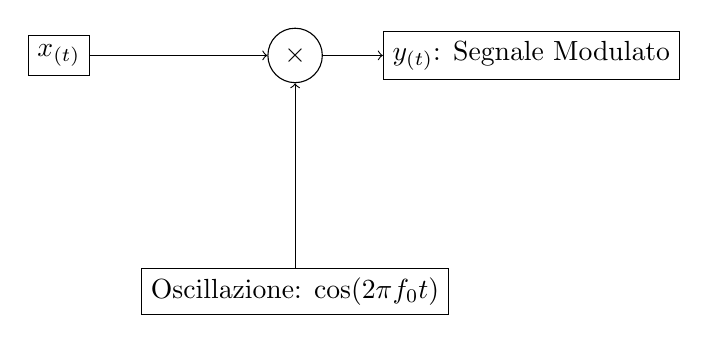
\begin{tikzpicture}[
                        node distance=3cm
                    ]
                    % Blocks
                    \node [rectangle, draw] (input) {$x_{(t)}$};
                    \node [circle, draw, right of=input] (product) {$\times$};
                    \node [rectangle, draw, below of=product] (carrier) {Oscillazione: $\cos(2\pi f_0t)$};
                    \node [rectangle, draw, right of=product] (modulated) {$y_{(t)}$: Segnale Modulato};
                
                    % Connections
                    \draw [->] (input) -- (product);
                    \draw [->] (product) -- (modulated);
                    \draw [->] (carrier) -- (product);
                \end{tikzpicture}    
                \label{fig:sistema di modulazione}
            }
            \hfill
            \subfloat[{\color{blue}$x_{(t)}$}, {\color{red}$y_{(t)}$}, {\color{purple}$\cos (2\pi t)$}]{
                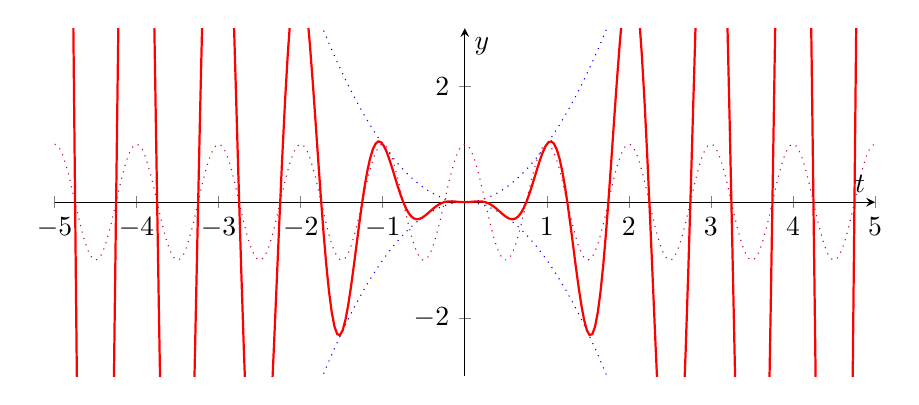
\begin{tikzpicture}
                    \begin{axis}[
                        domain=-5:5,
                        samples=200,
                        axis lines=middle,
                        xlabel=$t$,
                        ylabel=$y$,
                        ymin=-3,
                        ymax=3,
                        width=12cm,
                        height=6cm
                    ]
                    \addplot [blue, dotted, samples = 300] {(x^2)};
                    \addplot [blue, dotted, samples = 300] {-(x^2)};
                    \addplot [purple,dotted, samples = 300] {cos(deg(2*pi*x))};
                    \addplot [red, thick, samples = 300] {cos(deg(2*pi*x))*(x^2)};
                    \end{axis}
                \end{tikzpicture}
                \label{fig:modulazione in ampiezza}
            }
            \caption{Esempio sistema di modulazione di ampiezza}
        \end{figure}
        L'oscillazione introdotta, $\cos (2\pi t)$, segue l'andamento di $x_{(t)}$
        Nel dominio della frequenza:
        \begin{figure}[H]
            \centering
            \subfloat[Senza modulazione]{
                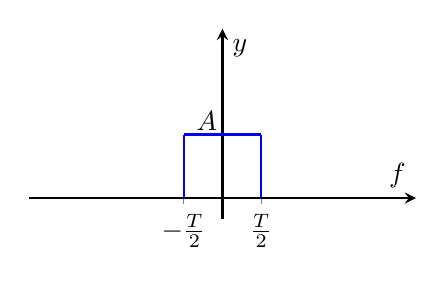
\begin{tikzpicture}
                    \begin{axis}[
                        xlabel=$f$,
                        ylabel=$y$,
                        xmin=-5,
                        xmax=5,
                        ymin=-0.5,
                        ymax=4,
                        ytick = {1.5},
                        xtick={-1, 0, 1},
                        xticklabels={$-\frac{T}{2}$, $0$, $\frac{T}{2}$},
                        yticklabels = {$A$},
                        yticklabel style = {yshift=5pt,xshift=4pt}, 
                        axis lines=middle,
                        thick,
                        domain=-5:5,
                        samples=100,
                        width=6.5cm,
                        height=4cm
                    ]
                    \addplot [const plot, blue, thick] coordinates{(-1,1.5)(1,1.5)};
                    \addplot [const plot, blue, thick] coordinates{(-1,0)(-1,1.5)};
                    \addplot [const plot, blue, thick] coordinates{(1,0)(1,1.5)};
                
                    \end{axis}
                \end{tikzpicture}
                \label{fig:segnale senza modulazione}
            }
            \hfill
            \subfloat[Con modulazione]{
                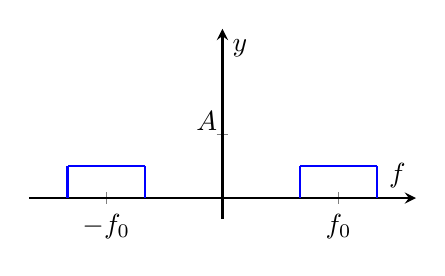
\begin{tikzpicture}
                    \begin{axis}[
                        xlabel=$f$,
                        ylabel=$y$,
                        xmin=-5,
                        xmax=5,
                        ymin=-0.5,
                        ymax=4,
                        ytick = {1.5},
                        xtick={-3,0,3},
                        xticklabels={$-f_0$, $0$,$f_0$},
                        yticklabels = {$A$},
                        yticklabel style = {yshift=5pt,xshift=4pt}, 
                        axis lines=middle,
                        thick,
                        domain=-5:5,
                        samples=100,
                        width=6.5cm,
                        height=4cm
                    ]
                    \addplot [const plot, blue, thick] coordinates{(-2,0.75)(-4,0.75)};
                    \addplot [const plot, blue, thick] coordinates{(-2,0)(-2,0.75)};
                    \addplot [const plot, blue, thick] coordinates{(-4,0)(-4,0.75)};
                    
                    \addplot [const plot, blue, thick] coordinates{(2,0.75)(4,0.75)};
                    \addplot [const plot, blue, thick] coordinates{(2,0)(2,0.75)};
                    \addplot [const plot, blue, thick] coordinates{(4,0)(4,0.75)};
                    
                    \end{axis}
                \end{tikzpicture}
                \label{fig:segnale con modulazione}
            }
            \caption{Segnale nel dominio della frequenza modulato e non}
        \end{figure}
        Serve per spostare la frequenza (es. di trasmissione) del segnale in modo tale, ad esempio, da non sovrapporre due segnali che sono sulla stessa frequenza.
        Se il segnale non fosse modulato si dice in {\color{blue} \textbf{banda base} (BB)} se il segnale é modulato si dice in {\color{red}\textbf{banda passante}(BP)}.
        \begin{figure}[H]
            \centering
            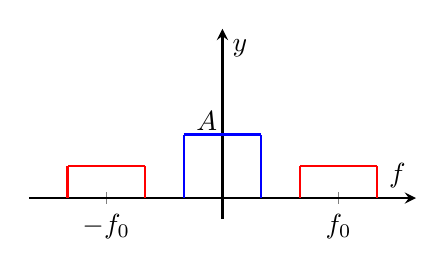
\begin{tikzpicture}
                \begin{axis}[
                    xlabel=$f$,
                    ylabel=$y$,
                    xmin=-5,
                    xmax=5,
                    ymin=-0.5,
                    ymax=4,
                    ytick = {1.5},
                    xtick={-3,0,3},
                    xticklabels={$-f_0$, $0$,$f_0$},
                    yticklabels = {$A$},
                    yticklabel style = {yshift=5pt,xshift=4pt}, 
                    axis lines=middle,
                    thick,
                    domain=-5:5,
                    samples=100,
                    width=6.5cm,
                    height=4cm
                ]
                \addplot [const plot, red, thick] coordinates{(-2,0.75)(-4,0.75)};
                \addplot [const plot, red, thick] coordinates{(-2,0)(-2,0.75)};
                \addplot [const plot, red, thick] coordinates{(-4,0)(-4,0.75)};
                
                \addplot [const plot, red, thick] coordinates{(2,0.75)(4,0.75)};
                \addplot [const plot, red, thick] coordinates{(2,0)(2,0.75)};
                \addplot [const plot, red, thick] coordinates{(4,0)(4,0.75)};
            
                \addplot [const plot, blue, thick] coordinates{(-1,1.5)(1,1.5)};
                \addplot [const plot, blue, thick] coordinates{(-1,0)(-1,1.5)};
                \addplot [const plot, blue, thick] coordinates{(1,0)(1,1.5)};
            
                
                \end{axis}
            \end{tikzpicture}
            \caption{{\color{blue}BB}, {\color{red}BP}}
            \label{fig:bb e bp}
        \end{figure}

        \subsubsection{Th. Modulazione con $\cos(2\pi f_0t)$}\label{Modulazione con coseno}
            $Ip:\begin{cases}
                    y_{(t)}= x_{(t)}\cos(2\pi f_0t)\\        
                    x_{(t)}\rightleftharpoons^{TCF} X_{(f)}
                \end{cases}$\\
            $Th: Y_{(f)} = \frac{1}{2} X_{(f-f_0)} + \frac{1}{2} X_{(f+f_0)}$ \\
            Dimostrazione:
            \begin{align}
                Y_{(f)} & = \int_{-\infty}^{\infty} y_{(t)} e^{-j2\pi ft} dt = \int_{-\infty}^{\infty} x_{(t)}\cos(2\pi f_0t) e^{-j2\pi ft} dt \nonumber \\
                & =\int_{-\infty}^{\infty} x_{(t)} \frac{e^{j2\pi f_0t} + e^{-j2\pi f_0t}}{2} e^{-j2\pi ft} dt =  \nonumber \\
                & = \frac{1}{2} \int_{-\infty}^{\infty} x_{(t)} e^{-j2\pi (f-f_0)t} dt + \frac{1}{2} \int_{-\infty}^{\infty} x_{(t)} e^{-j2\pi (f+f_0)t} dt \nonumber \\
                & = \eval{TCF[x_{(t)}]}_{f-f_0} + \eval{TCF[x_{(t)}]}_{f+f_0} = \frac{1}{2} X_{(f-f_0)} + \frac{1}{2} X_{(f+f_0)}\ c.v.d \nonumber  
            \end{align}
            Esempio:\\
            {
                $X_{(f)} = \frac{A}{B}rect\left(\frac{f}{B}\right)$
                \[
                    Y_{(f)} = \frac{A}{2B}rect\left(\frac{f-f_0}{B}\right)+\frac{A}{2B}rect\left(\frac{f+f_0}{B}\right)
                \]
                \begin{figure}[H]
                    \centering
                    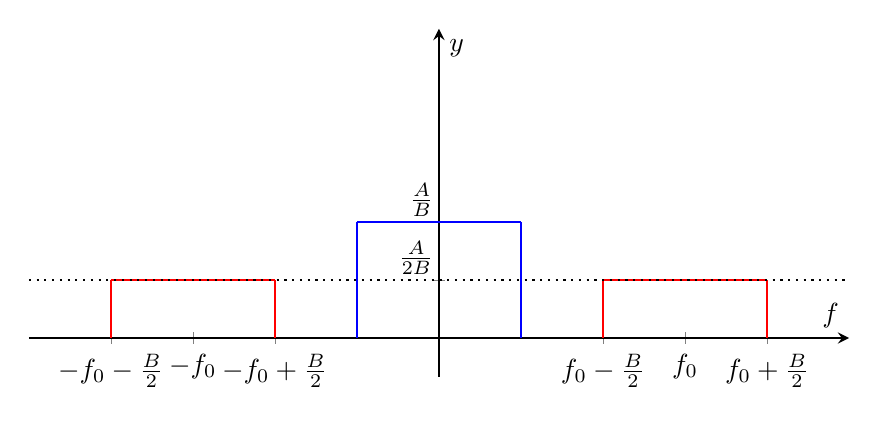
\begin{tikzpicture}
                        \begin{axis}[
                            xlabel=$f$,
                            ylabel=$y$,
                            xmin=-5,
                            xmax=5,
                            ymin=-0.5,
                            ymax=4,
                            ytick = {0.75,1.5},
                            xtick={-4,-3,-2, 0,2,3,4},
                            xticklabels={$-f_0-\frac{B}{2}$,$-f_0$,$-f_0+\frac{B}{2}$,$0$,$f_0-\frac{B}{2}$,$f_0$,$f_0+\frac{B}{2}$},
                            yticklabels = {$\frac{A}{2B}$,$\frac{A}{B}$},
                            yticklabel style = {yshift=8pt,xshift=4pt}, 
                            axis lines=middle,
                            thick,
                            domain=-5:5,
                            samples=100,
                            width=12cm,
                            height=6cm
                        ]
                        \addplot [const plot, red, thick] coordinates{(-2,0.75)(-4,0.75)};
                        \addplot [const plot, red, thick] coordinates{(-2,0)(-2,0.75)};
                        \addplot [const plot, red, thick] coordinates{(-4,0)(-4,0.75)};
                        
                        \addplot [const plot, red, thick] coordinates{(2,0.75)(4,0.75)};
                        \addplot [const plot, red, thick] coordinates{(2,0)(2,0.75)};
                        \addplot [const plot, red, thick] coordinates{(4,0)(4,0.75)};
                    
                        \addplot [const plot, blue] coordinates{(-1,1.5)(1,1.5)};
                        \addplot [const plot, blue] coordinates{(-1,0)(-1,1.5)};
                        \addplot [const plot, blue] coordinates{(1,0)(1,1.5)};
                        
                        \addplot [const plot,dotted, black] coordinates{(-5,0.75)(5,0.75)};

                        \end{axis}
                    \end{tikzpicture}
                    \caption{{\color{blue}$X_{(f)}$}, {\color{red}$Y_{(f)}$}}
                    \label{fig:modulazione rect}
                \end{figure}
            }
            fai cosa ha chiesto lui a fine lezione
        \subsubsection{Th. Modulazione con $\sin(2\pi f_0t)$}\label{Modulazione con seno}
        $Ip:\begin{cases}
                y_{(t)}= x_{(t)}\sin(2\pi f_0t)\\        
                x_{(t)}\rightleftharpoons^{TCF} X_{(f)}
            \end{cases}$\\
        $Th: Y_{(f)} = \frac{1}{2j} X_{(f-f_0)} - \frac{1}{2j} X_{(f+f_0)} $ \\
        Dimostrazione: 
        \begin{align}
            Y_{(f)} & = \int_{-\infty}^{\infty} y_{(t)} e^{-j2\pi ft} dt = \int_{-\infty}^{\infty} x_{(t)}\sin(2\pi f_0t) e^{-j2\pi ft} dt \nonumber \\
            & =\int_{-\infty}^{\infty} x_{(t)} \frac{e^{j2\pi f_0t} - e^{-j2\pi f_0t}}{2j} e^{-j2\pi ft} dt =  \nonumber \\
            & = \frac{1}{2j} \int_{-\infty}^{\infty} x_{(t)} e^{-j2\pi (f-f_0)t} dt - \frac{1}{2j} \int_{-\infty}^{\infty} x_{(t)} e^{-j2\pi (f+f_0)t} dt \nonumber \\
            & = \eval{TCF[x_{(t)}]}_{f-f_0} - \eval{TCF[x_{(t)}]}_{f+f_0} = \frac{1}{2j} X_{(f-f_0)} - \frac{1}{2j} X_{(f+f_0)}\ c.v.d \nonumber  
        \end{align}

        \subsubsection{Th. Modulazione con $\cos(2\pi f_0t + \phi)$}\label{Modulazione con coseno generico}
            $Ip: \begin{cases}
                y_{(t)}= x_{(t)}\cos(2\pi f_0t + \phi)\\        
                x_{(t)}\rightleftharpoons^{TCF} X_{(f)}
                \end{cases}$\\
            $Th: Y_{(f)} = \frac{e^{j\phi}}{2} X_{(f-f_0)} + \frac{e^{-j\phi}}{2} X_{(f+f_0)} $ \\
            Dimostrazione: 
            \begin{align}
                Y_{(f)} & = \int_{-\infty}^{\infty} y_{(t)} e^{-j2\pi ft} dt = \int_{-\infty}^{\infty} x_{(t)}\cos(2\pi f_0t + \phi) e^{-j2\pi ft} dt \nonumber \\
                & =\int_{-\infty}^{\infty} x_{(t)} \frac{e^{j(2\pi f_0t+ \phi)} + e^{-j(2\pi f_0t+ \phi)}}{2} e^{-j2\pi ft} dt =  \nonumber \\
                & = \frac{e^{j\phi}}{2} \int_{-\infty}^{\infty} x_{(t)} e^{-j2\pi (f-f_0)t} dt + \frac{e^{-j\phi}}{2} \int_{-\infty}^{\infty} x_{(t)} e^{-j2\pi (f+f_0)t} dt \nonumber \\
                & = \eval{TCF[x_{(t)}]}_{f-f_0} + \eval{TCF[x_{(t)}]}_{f+f_0} = \frac{e^{j\phi}}{2} X_{(f-f_0)} + \frac{e^{-j\phi}}{2} X_{(f+f_0)}\ c.v.d \nonumber  
            \end{align}
            Esempio:
            \begin{figure}[H]
                \centering
                \subfloat[Ampiezza Mod. generica]{
                    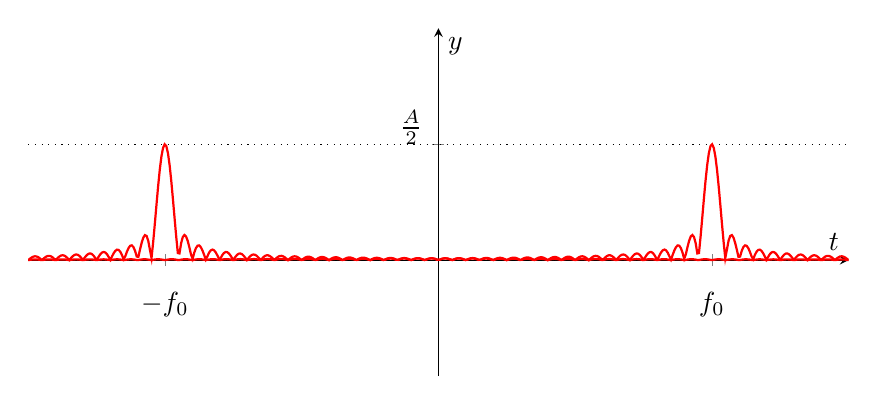
\begin{tikzpicture}
                        \begin{axis}[
                            domain=-30:30,
                            samples=200,
                            axis lines=middle,
                            xlabel=$t$,
                            ylabel=$y$,
                            ytick = {0.5},
                            yticklabels = {$\frac{A}{2}$},
                            yticklabel style = {yshift=6pt},
                            xtick = {-20,20},
                            xticklabels = {$-f_0$,$f_0$},
                            xticklabel style = {yshift=-6pt}, 
                            ymin=-0.5,
                            ymax=1,
                            width=12cm,
                            height=6cm
                        ]
                        \addplot [const plot, dotted,black] coordinates{(-30,0.5)(30,0.5)};
                        \addplot [red, thick, samples = 500] {abs(sin(deg((x-20)*pi))/(2*(x-20)*pi))};
                        \addplot [red, thick, samples = 500] {abs(sin(deg((x+20)*pi))/(2*(x+20)*pi))};
                        \end{axis}
                    \end{tikzpicture}
                    \label{fig:Ampiezza Mod. generica}
                }
                \hfill
                \subfloat[fase Mod. generica]{
                        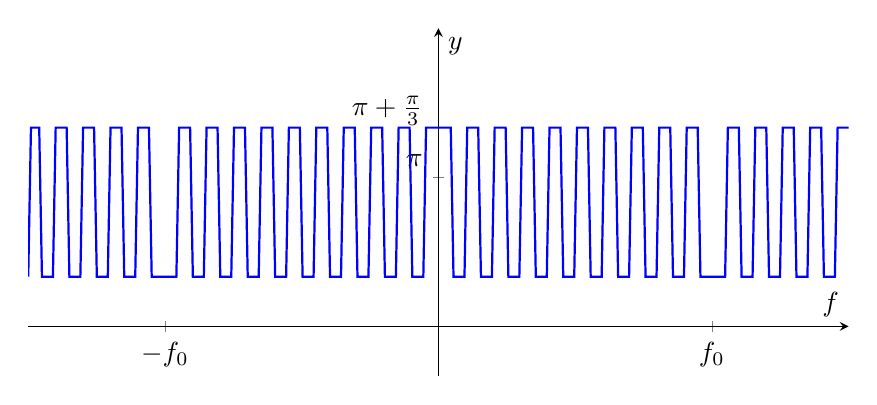
\begin{tikzpicture}
                            \begin{axis}[
                                domain=-30:30,
                                samples=200,
                                axis lines=middle,
                                xlabel=$f$,
                                ylabel=$y$,
                                ymin=-pi/3,
                                ymax=2*pi,
                                xtick={-20,20},
                                xticklabels={$-f_0$,$f_0$},
                                ytick={pi,pi+(pi*1/3)},
                                yticklabel style = {yshift=6pt}, 
                                yticklabels={$\pi$,$\pi+\frac{\pi}{3} $},
                                width=12cm,
                                height=6cm
                            ]
                            \addplot [blue, thick, samples = 300] {rad(atan2(0,(x*sin(deg(pi*x)))/(pi*(-400 + x^2))))+(pi*1/3)};
                            \end{axis}
                        \end{tikzpicture}
                    \label{fig:fase Mod. generica}
                }
                \caption{Modulazione generica di una $A rect\left(\frac{t}{T}\right)$ con $\cos(2\pi f_0t+\frac{\pi}{3})$}
            \end{figure}
        É legale cosa ho scritto sopra della modulazione generica?
        \subsubsection{Th. Modulazione con Esponenziale Complesso}\label{Modulazione con Esponenziale Complesso}
            $Ip: \begin{cases}
                y_{(t)}= x_{(t)}e^{j2\pi f_0t}\\        
                x_{(t)}\rightleftharpoons^{TCF} X_{(f)}
                \end{cases}$\\
            $Th: Y_{(f)} = X_{(f-f_0)} $ \\
            Dimostrazione: 
            \begin{align}
                Y_{(f)} & = \int_{-\infty}^{\infty} y_{(t)} e^{-j2\pi ft} dt = \int_{-\infty}^{\infty} x_{(t)}e^{j2\pi f_0t} e^{-j2\pi ft} dt \nonumber \\
                & =\int_{-\infty}^{\infty} x_{(t)} e^{-j2\pi (f-f_0)t} dt = \eval{TCF[x_{(t)}]}_{f-f_0} = X_{(f-f_0)} \nonumber
            \end{align}
            Posso notare che:
            \begin{itemize}
                \item Ritardo: $\rightarrow x_{(t-t_0)} \rightleftharpoons X_{(f)} e^{(-j2\pi ft_0)}$
                \item Modulazione: $\rightarrow x_{(t)}e^{(j2\pi f_0t)} \rightleftharpoons X_{(f-f_0)}$
            \end{itemize}
            Procedimento per la sintesi di un segnale:
            \begin{itemize}
                \item Derivo il segnale
                \item Verifico le ipotesi del Th. dell'Integrazione \ref{Integrazione}
                \item calcolo la TCF della derivata
                \item Applico il Th. dell'integrazione per calcolare $X_{(f)}$
            \end{itemize}